\section{Decisões de Projeto}
\label{sec:project}
O sistema proposto está disponível em \, \url{https://github.com/pantuza/pox}.
Seguindo o design do POX, 
o módulo de grafos (\emph{graph}) se integra com 
os eventos relacionados à infraestrutura da rede,
que foram unificados no \emph{topology} e no \emph{host\_tracker}.
A integração do módulo \emph{graph} ocorre conforme a figura \ref{fig:design}.

\begin{figure}[h!]
    \centering
    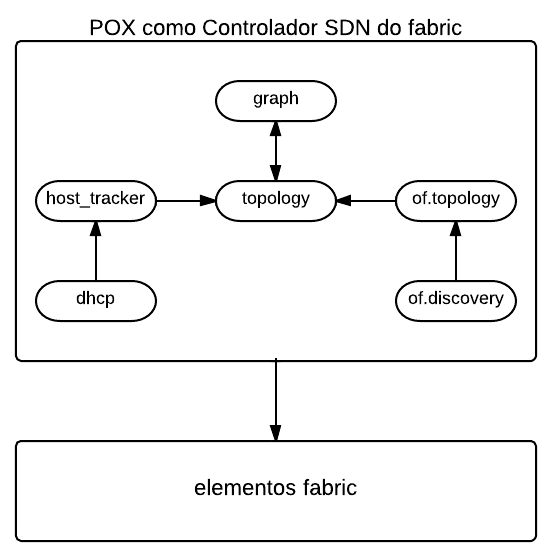
\includegraphics[scale=0.4]{fabric_design.png}
    \caption{integração entre os módulos}
    \label{fig:design}
\end{figure}

Seguem-se as principais decisões de projeto na implementação do sistema.

\subsection{Integração do \emph{host\_tracker} com o \emph{topology} e o \emph{misc.dhcpd}}

O \emph{host\_tracker} foi alterado para 
comunicar com o \emph{topology} através dos eventos de 
adicão ({\it join}) e remoção ({\it leave}) dos {\it hosts}. 
O \emph{host\_tracker}, ao descobrir mudanças no estado dos \emph{hosts} da rede, 
notifica o \emph{topology}. 
Por sua vez, o \emph{topology}, ao perceber mudanças na topologia da rede, 
informa o \emph{graph}, via evento, para que o grafo seja atualizado. 

Em suas contribuições recentes, o POX recebeu um módulo de DHCP. 
Esse módulo dispara eventos de \emph{DHCPLease} para o \emph{core} 
ao associar um IP para um \emph{host}.
Foi adicionado ao \emph{host\_tracker} um método para fazer escuta desse evento. 
Ao ser notificado, 
o método atualiza o dicionário python que mantém as informações dos hosts ativos. 
Essa alteração possibilita a descoberta antecipada de novos hosts na rede, 
otimizando a tarefa do \emph{host\_tracker}.

A integração entre \emph{host\_tracker} e \emph{topology} 
foi feita utilizando a estrutura de eventos que o POX possui. 
Assim, quando \emph{host\_tracker} recebe um evento de PacketIn, 
ele dispara um evento para o \emph{topology}, 
de maneira que o mesmo trate a entrada de um host na topologia da rede.
Esse evento (\emph{HostEvent}) foi implementado dentro do módulo \emph{topology} 
com o objetivo de manter a semântica por entidades (\emph{entity}). 
Assim, ao adicionar uma entidade ao \emph{topology}, se essa entidade é uma 
instância da classe \emph{Host}, então dispara-se o evento \emph{HostEvent}. 
O mesmo funcionamento é utilizado para a descoberta de \emph{switches} feita pelo
módulo \emph{openflow.topology} (módulo para descoberta de switches openflow)
que adiciona uma entidade da classe \emph{Switch} ao \emph{topology}.

Quando um vértice se torna inativo o módulo \emph{graph} é notificado
pelos módulos \emph{host\_tracker} e \emph{openflow.topology}.
Quando um \emph{switch} torna-se inativo, um evento de 
\emph{SwitchLeave} é disparado pelo \emph{openflow.topology} e o
módulo \emph{graph} pode atualizar o grafo representando a rede.
Essa identificação é feita através do protocolo LLDP e o evento 
é disparado imediatamente e o grafo atualizado.
Por sua vez, quando um \emph{host} está inativo, é necessário 
perguntar ao \emph{host} se ele ainda está ativo. 
Esse procedimento é feito pelo \emph{host\_tracker} que envia 
pacotes ARP para verificar a atividade do \emph{host}. 
Essa identificação é configurada no módulo \emph{host\_tracker}
que pode decidir a quantidade de pacotes ARP e a periodicidade 
dessa verificação. 
Assim, ao ser identificado que um \emph{host} está inativo 
o grafo é atualizado.

\subsection{Ajustes para incluir eventos relacionados com as arestas do grafo}

As arestas entre os \emph{hosts} e \emph{switches} são obtidas
indiretamente pelo evento de entrada e saída de \emph{host},
pressupondo um link necessário com o \emph{switch} diretamente conectado.
Nesse caso, é fundamental que o \emph{host\_tracker} informe 
o \emph{switch}, preferencialmente com o id 
ou o próprio objeto ``entidade'' do \emph{topology} e a porta da conexão.
Além disso, deve haver garantia que o \emph{host\_tracker} 
informe eventos de \emph{host} apenas quando estiver conectado
diretamente com o \emph{switch}.
Essas garantias já são consideradas na atual versão do \emph{host\_tracker}.

Outra forma de aresta do grafo ocorre entre os \emph{switches}.
Atualmente, o módulo \emph{openflow.discovery} controla os 
links entre \emph{switches} OpenFlow. 
Ele publica o evento \emph{LinkEvent} que notifica 
a entrada ({\it up} ou descoberta) e saída ({\it down} ou deleção)
dos links.
O módulo \emph{openflow.topology} atua como {\it subscriber} desse evento
e faz as atualizações necessárias nos dados do \emph{switch}.
Contudo, essa mudança de estado não é notificada para o \emph{topology}.
Esse é um ponto que foi necessário modificar a interface e os
eventos do \emph{topology}.
Para isso, foi adicionada a ``entidade'' \emph{Link} (subclasse) e
os eventos \emph{LinkJoin} e \emph{LinkLeave}.
O objeto \emph{Link} é composto de duas portas,
uma de cada \emph{Entity} conectada,
no caso, apenas \emph{switches}.


\subsection{Modelagem do grafo}
O grafo proposto pelo presente trabalho é representado por
$G=(V,A)$, no qual $V$ e $A$ são os conjuntos de vértices e arestas, respectivamente. 
 $V$ e $A$, são finitos.
Cada vértice $v \in V$ pode representar um \emph{host} ou um
\emph{switch} na rede. 
Cada aresta $u \to v \in A$ representa um link entre dois vértices.
As arestas possuem um peso $g(u, v)$ que descreve o volume de 
tráfego em bytes recebidos e transmitidos através da aresta/\emph{link}. 

Cada vértice é um objeto das classes \emph{Host} ou \emph{Switch},
logo, por herança são objetos da classe \emph{Entity}. 
Em função disso é possível identificar dentro do módulo 
\emph{graph} qual o tipo do vértice corrente. 
O peso das arestas é obtido através da leitura dos contadores 
de fluxos presentes nos \emph{switches openflow}.
Para o módulo \emph{graph} são lidos os contadores de fluxo da porta 
no switch. 
A lista de contadores é apresentada na Tabela \ref{tbl:counters} e em 
\citep{openflow2013protocol}.
Através da contagem desses fluxos é possível mensurar o tráfego 
decorrente na aresta/\emph{link}.

\begin{table}[h!]
    \centering
    \begin{tabular}{| l | l |}
    \hline
    \textbf{Contador} & \textbf{Bits} \\ \hline
    Pacotes Recebidos & 64 \\ \hline
    Pacotes Transmitidos & 64 \\ \hline
    Bytes Recebidos & 64 \\ \hline
    Bytes Transmitidos & 64 \\ \hline
    Drops Recebidos & 64 \\ \hline
    Drops Transmitidos & 64 \\ \hline
    Erros Recebidos & 64 \\ \hline
    Erros Transmitidos & 64 \\ \hline
    Erros de Frames Recebidos & 64 \\ \hline
    Erros de Transbordo Transmitidos & 64 \\ \hline
    Erros de CRC Recebidos & 64 \\ \hline
    Colisões & 64 \\
    \hline
    \end{tabular}
    \caption{Contadores de fluxos por Porta}
    \label{tbl:counters}
\end{table}

\subsection{Elaboração do módulo \emph{graph}}

As modificações descritas completam os requisitos necessário para o módulo \emph{graph},
em especial o controle de eventos que afetam os vértices e arestas do grafo.
Através das informações topológicas fornecidas pelos eventos do \emph{topology},
a classe \emph{graph} mantém, em memória, um grafo atualizado em tempo real. 
A instância dessa classe é \emph{subscriber} dos eventos do módulo \emph{topology}. 
Dessa forma, recebe-se eventos de qualquer um dos {\it publishers} 
do canal de eventos canônico do \emph{topology}, 
incluindo o \emph{openflow\_discovery} e \emph{host\_tracker}. 

\subsection{Interface de programação (API)}

O \emph{graph} possui uma interface (API) para que outros módulos do 
controlodor possam requisitar informações da topologia da rede. 
É possível imaginar aplicações como balanceamento de carga ou roteamento
que utilizem informações contidas no grafo.

\begin{outline}
\0 Os Métodos com dados do grafo são:
    \1 \emph{get\_vertex(id)}:
    Retorna uma entidade do grafo identificada (id dado pelo \emph{topology}).
    \1 \emph{get\_adjacents(id)}: 
    Retorna os nós (vértices) imediatamente adjacentes ao nó com identificado.
    \1 \emph{snapshot()}: 
    Retorna uma cópia do grafo, em forma de duas coleções, 
    uma de vértices (nós) e outra de arestas.
    \1 \emph{to\_dot(harq, layout = "dot")}: 
    Grava uma cópia do grafo para ser processada pelo Graphviz
    \citep{john2003graphviz}.
\0 Os Algoritmos de grafos já implementados são:
    \1 \emph{get\_mst()}:
    Retorna uma árvore geradora mínima do grafo (\emph{minimum spanning tree})
    em tempo real. A árvore é computada sempre que o grafo é atualizado.
\end{outline}


\subsection{Simulação via Mininet}

O funcionamento do módulo \emph{graph} do POX foi testado no Mininet,
\citep{lantz2010network}
um software de simulação de rede amplamente usado, 
principalmente para controladores SDN.
O Mininet, assim como o POX, é implementado em Python.
Também foi necessário acrescentar recursos para viabilizar o uso do Mininet,
especialmente métodos de adição e remoção de elementos na rede,
uma vez que os grafos devem ser mantidos de forma dinâmica.
Apesar de ser amplamente programável, 
as remoções e inserções dinâmicas de entidades de rede 
não eram disponibilizadas no Mininet,
principalmente depois de estabelecida a topologia inicial 
e da rede entrar em funcionamento.
Boa parte do esforço  análise detalhada dos algoritmos e das estruturas de dados usadas 
no controle do Mininet, foram implementados e testados diversos métodos.
A compatibilidade também foi o principal fator das alterações feitas,
mantendo-se sempre as estruturas e interfaces originais do Mininet.
Além das interfaces de código, que tiveram reflexo em várias classes, 
a interface de comandos padrão (\emph{prompt}) do Mininet
foi estendida para os novos comandos de adição e remoção dinâmica de controladores,
 \emph{switches}, \emph{hosts}, \emph{links} e interfaces de rede.